\documentclass[./Research.tex]{subfiles}

\begin{document}

 Consider the construction of a neural network to alternately add and subtract numbers. It is useful to represent all binary operations in list form, $\left(+\;a\;b\right)$. The neural network, then, becomes a representation of a stack. 

\def\layersep{2.5cm}

\vspace{2em}
{\centering
\begin{tikzpicture}[shorten >=1pt,->,draw=black!50, node 
distance=\layersep]

    \tikzstyle{every pin edge}=[<-,shorten <=1pt]
    \tikzstyle{neuron}=[circle,fill=black!25,minimum size=17pt,inner sep=0pt]
    \tikzstyle{input neuron}=[neuron, fill=green!50];
    \tikzstyle{output neuron}=[neuron, fill=red!50];
    \tikzstyle{hidden neuron}=[neuron, fill=blue!50];
    \tikzstyle{annot} = [text width=4em, text centered]

 
    % Draw the hidden layer nodes
    \foreach \name / \y / \symbol in {1/1/+,2/2/a,3/3/-}
        \path[yshift=0.5cm]
            node[hidden neuron] (H-\name) at (\layersep,-\y cm) {\symbol};

    % Draw the output layer node
    \node[output neuron,pin={[pin edge={->}]right:$\left(+\;a\;b\right)$}, right of=H-3] (O) {\texttt{eval(}$\left(+\;a\;b\right)$\texttt{)}};

    % Connect every node in the hidden layer with the output layer
    \foreach \source in {1,...,3}
        \path (H-\source) edge (O);

    % Annotate the layers
    \node[annot,left of=H-1] {Input};
\end{tikzpicture}
}


\includegraphics[scale=1]{Visuals/NeuralNetwork_1_NetworkTree.ps} \\

This tree-like structure closely mimics the abstract syntax tree which is generated by compilers when processing code in a program. For example, to evaluate the results of the expressions "+ 5 4" and "- 5 4", a compiler may generate the following trees: \\

\includegraphics[scale=1]{Visuals/NeuralNetwork_1_SyntaxTree.ps}

{\color{red}
   To improve this sentence don't use \emph{weasel words}. I don't know what \emph{very similar} means to you. Neither a compiler nor interpreter \emph{view} code. Neither are (yet) sentient beings. 
   
   The best piece of writing advice I can give is: 
   \begin{quote}
       Mean exactly what you write and write exactly what you mean. 
   \end{quote}
}
\end{document}
